\documentclass[main.tex]{subfiles}

\begin{document}
    \section{Übersicht}
    Die Infrastruktur von CodeUp besteht aus mehreren Servern, die alle einen bestimmten Zweck erfüllen.
    Abbildung~\ref{fig:codeup-infra} zeigt die gesamte Infrastruktur von CodeUp und die Kommunikation zwischen den einzelnen Komponenten.
    \\

    \begin{figure}[h]
        \centering
        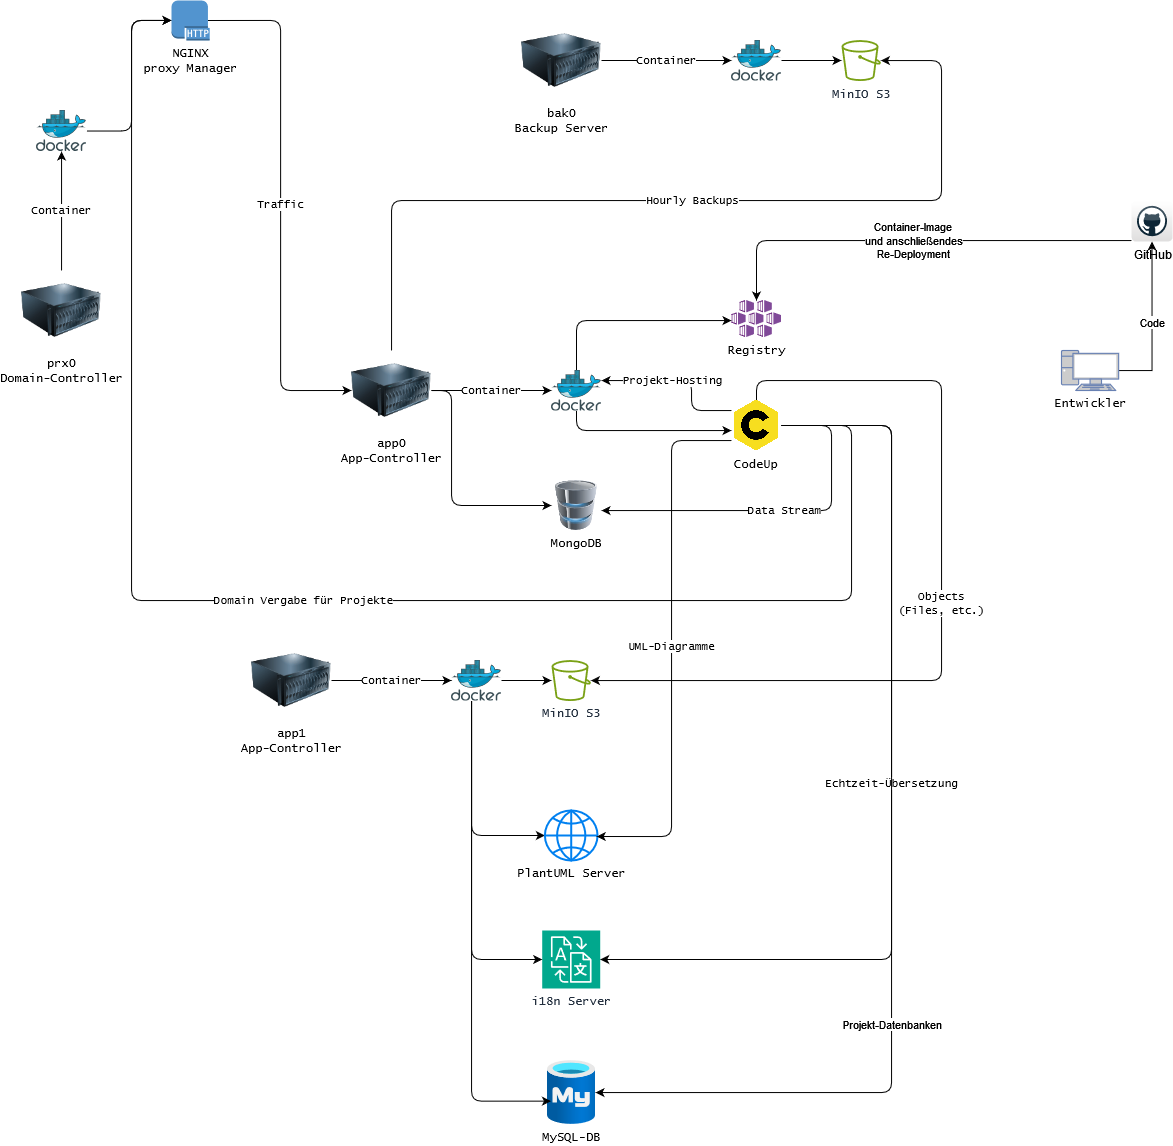
\includegraphics[width=0.75\textwidth]{assets/CodeUp-Infra}
        \caption{CodeUp-Infrastruktur}
        \label{fig:codeup-infra}
    \end{figure}
    \vspace{1em}
    Wie in der Abbildung zu sehen besteht die Infrastruktur aus vier Servern:
    \begin{itemize}
        \item \textbf{prx0 (Proxy-Server)}: Der Proxy-Server ist der Einstiegspunkt für alle Anfragen an CodeUp.
        Er leitet die Anfragen an die entsprechenden Server weiter und kümmert sich ebenfalls um die Domain-Vergabe für Projekte von Benutzern.
        Ebenfalls ist der Proxy-Server für die Verschlüsselung des Datenverkehrs mittels SSL-Zertifikaten zuständig.
        \item \textbf{bak0 (Backup-Server)}: Der Backup-Server hat die Aufgabe Backups von allen anderen Servern zu speichern und im Notfall wiederherzustellen.
        Für eine übersichtlichere Darstellung zeigt Abbildung~\ref{fig:codeup-infra} nur den Backup-Prozess des Hauptservers (app0), allerdings machen alle Server stündliche Backups, die auf dem Backup-Server gespeichert werden.
        \item \textbf{app0 (Application-Server)}: Der Application-Server ist der Hauptserver von CodeUp und beinhaltet die gesamte Logik der Plattform.
        Dieser ist der Dreh und Angelpunkt der Plattform und ist der einzige Server, bis auf den Proxy-Server mit dem der Benutzer direkt interagiert.
        Für einen schnelleren Datenverkehr ist die Hauptdatenbank auf diesem Server gespeichert.
        Der app0-Server ist ebenfalls für das Hosting der Projekte von Benutzern zuständig.
        Projekte werden auf diesem Server in einem Git-Repository gespeichert und ebenfalls regelmäßig auf den Backup-Server gesichert.
        \item \textbf{app1 (Application-Server)}: Der Application-Server app1 dient zum einen als Server für alle Services, die keine direkte Interaktion mit dem Benutzer benötigen und keine Daten speichern.
        Allerdings dient er auch als Objekt-Storage für Dateien, die Benutzer hochladen und stellt die Datenbanken für Benutzer-Projekte bereit.
    \end{itemize}
    \section{DevOps-Praktiken}
    Die Entwicklung und Bereitstellung von CodeUp wird durch DevOps-Praktiken erleichtert.
    Dies beinhaltet unter anderem die Automatisierung von Prozessen, die kontinuierliche Integration und Bereitstellung von Code und die Überwachung der Infrastruktur.
    \subsection{Automatisierung}
    Automatisierung ist ein wichtiger Bestandteil von DevOps und ermöglicht es, Prozesse zu beschleunigen und Fehler zu minimieren.
    Bei CodeUp ist der Bereitstellungsprozess vollständig automatisiert, sodass neue Versionen der Plattform möglichst schnell und ohne menschliches Eingreifen bereitgestellt werden können.
    Dies funktioniert durch die Verwendung von GitHub-Actions, die bei jedem Push in das Haupt-Repository ein Container-Image von CodeUp erstellen und dieses anschließend in der Docker-Registry, welche auf dem Server app0 gehostet wird, speichern.
    Sollte das Image erfolgreich erstellt worden sein, wird es durch GitHub-Actions auf dem Server installiert und CodeUp wird mit dem neuen Image neu gestartet.
    \subsection{Überwachung}
    Die Überwachung der gesamten Infrastruktur findet auf den Servern prx0 und app1 statt.
    Diese überprüfen regelmäßig die Verfügbarkeit der anderen Server und senden im Falle eines Ausfalls eine Benachrichtigung an den Administrator.
    Alle Container sind so eingestellt, dass sie bei einem Absturz automatisch neu gestartet werden, um die Ausfallzeit zu minimieren.
    Die einzige menschliche Interaktion bei einem Ausfall ist die Überprüfung der Ursache und die Behebung des Problems.
    Gegebenenfalls muss ein Administrator die tatsächlichen Server neu starten oder im schlimmsten Fall auf ein Backup zurückgreifen.
    \section{Technologie Entscheidungen}
    Die Entscheidung für die einzelnen Technologien wurde aufgrund der Anforderungen an CodeUp getroffen.
    So wurde beispielsweise eine Microservice-Architektur gewählt, um die Skalierbarkeit und Wartbarkeit der Plattform zu gewährleisten.
    Ebenfalls wurde Docker als Container-Technologie gewählt, anstatt virtuelle Maschinen zu verwenden, um die Ressourcennutzung zu optimieren und die Bereitstellung von CodeUp zu vereinfachen.
    Die Wahl von MongoDB als Datenbank wurde getroffen, da sie eine hohe Flexibilität bietet und somit die Anforderungen an CodeUp erfüllt.
    Auch die Wahl von Node.js als Programmiersprache für die Server wurde getroffen, da sie eine hohe Performance bietet und die Entwicklung von CodeUp vereinfacht.
    Node.js ist zwar nicht die schnellste Programmiersprache, allerdings bietet sie eine hohe Skalierbarkeit und eine einfache Handhabung.
    Aus ähnlichen Gründen fiel die Wahl der Dateispeicherung auf MinIO, da es eine hohe Performance bietet und das Teilen von Dateien sehr einfach gestaltet.
    Für die Datenbanken von Benutzer-Projekten wurde MySQL gewählt, da es die SQL-Sprache unterstützt und somit gut in den schulischen Kontext eingebunden werden kann.
    Es wurde bewusst auf eine Cloud-Lösung, wie AWS oder GCP verzichtet, um Kosten so gering wie möglich zu halten und die Kontrolle über die Daten zu behalten.
    Allerdings ist die Infrastruktur von CodeUp so aufgebaut, dass eine spätere Migration in die Cloud möglich ist, sollte dies notwendig werden.
\end{document}
